\section{Development Grouping and Repetition Results}
\label{sec:findings}
The development comparison relates overall accuracy and inference cost to changes in individual judgments, repeat variability, and class-level effects. Figure~\ref{fig:development-map} places ten models by cost per contract and baseline accuracy; bubble area shows the fraction of anchors correct across all twelve follow-up responses. This fraction is available for Jev, both Qwen models, Flash-Lite, Terra, Sonnet, and Haiku. Gemini Pro and Luna have no development anchor observations, while Astra has only partial coverage, so their stability is marked unavailable rather than zero. Accuracy and all-twelve correctness describe complementary aspects of performance on different contract sets.
\begin{figure*}[t]
\centering
{\small\textbf{Development set: ten-model comparison}\par\medskip}
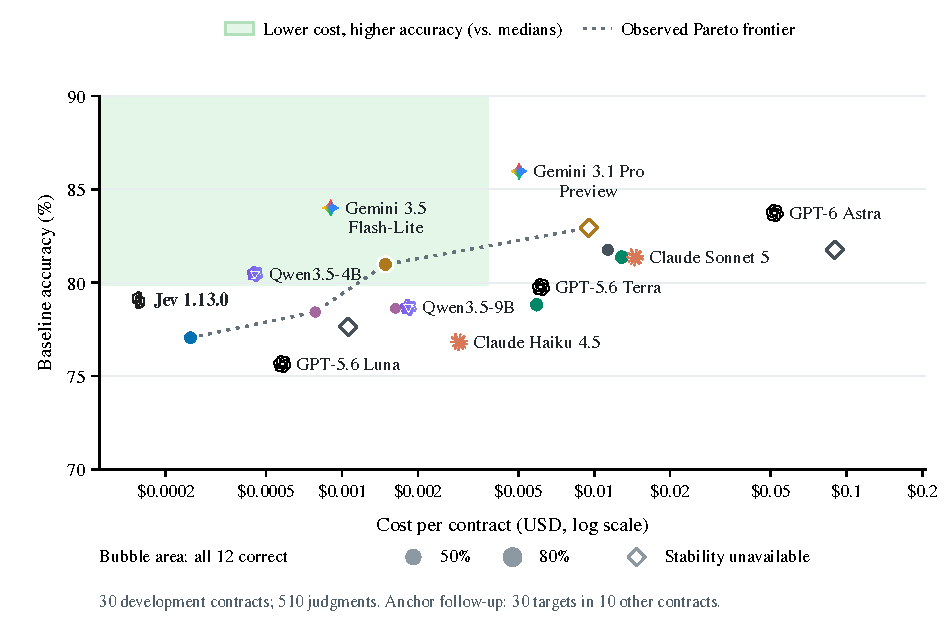
\includegraphics[width=0.92\textwidth]{figures/development_cost_accuracy.pdf}
\caption[Development comparison of cost, accuracy, and correctness across twelve responses.]{Cost, accuracy, and correctness across all twelve anchor responses describe complementary aspects of development performance. Point coordinates use 30 development contracts (510 judgments); bubble areas use 30 anchors from ten disjoint development contracts. A hollow diamond denotes an unmeasured or incomplete anchor evaluation, rather than zero stability. API costs use reported charges or recorded token usage at public rates; local costs use single-GPU rental equivalents at \$2 per GPU-hour. The green region marks cost below and accuracy above the ten-model medians (\$0.003767 and 79.90\%). The dotted frontier joins nondominated point estimates under these cost bases; it does not test significance. Astra's coordinates retain the historical OpenRouter evaluation.
}
\label{fig:development-map}
\end{figure*}
\subsection{Correctness and sensitivity are distinct}
Jev achieves 77.06\% accuracy, while Gemini Pro has the highest observed accuracy (82.94\%) and Macro-F1 (77.19\%) among the ten development baselines (Table~\ref{tab:baseline}). The added Terra, Sonnet, and Haiku baselines achieve 81.76\%, 81.37\%, and 78.82\% accuracy, respectively. At the stated prices, none extends the observed cost--accuracy frontier formed by Jev, Qwen4B, Flash-Lite, and Gemini Pro. Both the contracts and Qwen inference configurations differ between the development and test comparisons, preventing attribution of their frontier differences to either factor alone.

Similar aggregate accuracy can accompany substantial changes in individual judgments (Table~\ref{tab:stability30}). In the five-model comparison, Qwen4B changes 87/510 labels when moving from joint $K=17$ inference to $K=1$, but the number correct changes only from 399 to 395. These transitions comprise 38 regressions, 34 corrections, and 15 switches between wrong labels. Flash-Lite and Luna both change 68 labels, although their net numbers correct change by minus five and plus one. For Qwen9B, reordering the $K=17$ hypotheses changes 51 labels while reducing the number correct by one.

\textbf{Finding 1: Aggregate correctness can conceal substantial changes to individual decisions.} Across local and hosted generative models, corrections and regressions partly cancel in accuracy. Their separate counts distinguish beneficial changes from newly introduced errors.

\begin{table*}[t]
\centering
\small
\begin{tabular}{lrrrrrl}
\toprule
\rowcolor{tableHeader}
Model & $K{=}17$ & $K{=}1$ & $K$ flips & Order & Repeat & C$\to$W / W$\to$C / W$\to$W \\
\midrule
\rowcolor{jevRow}
\modelicon{jev}Jev 1.13.0 & 77.06 & 76.47 & 6 & 8 & 4 & 4 / 1 / 1 \\
\modelicon{qwen}Qwen3.5-4B & 78.24 & 77.45 & 87 & 83 & 0 & 38 / 34 / 15 \\
\modelicon{qwen}Qwen3.5-9B & 78.63 & 75.49 & 74 & 51 & 0 & 38 / 22 / 14 \\
\modelicon{gemini}Gemini 3.5 Flash-Lite & 80.98 & 80.00 & 68 & 30 & 16 & 33 / 28 / 7 \\
\modelicon{openai}GPT-5.6 Luna & 78.63 & 78.82 & 68 & 30 & 14 & 29 / 30 / 9 \\
\bottomrule
\end{tabular}
\caption{Development-set sensitivity to judgment-set size, order, and repetition on 30 contracts. Accuracy is reported in percentages; flip counts use 510 paired targets. Each model is compared with its own $K{=}17$ baseline. The final column decomposes the $K{=}17\to1$ transitions, where C/W denotes correctness rather than entailment class. Order and Repeat each represent one perturbation.}
\label{tab:stability30}
\end{table*}


\subsection{Repetition and class effects matter}
\paragraph{Repetition provides a reference for request changes.}
Jev shows few changes under grouping and permutation, but unchanged repetition also changes some labels. It changes 6/510 labels for $K17\to K1$, eight under permutation, and four under unchanged repetition (Figure~\ref{fig:controls}, Appendix~\ref{app:full}). All four targets that change under repetition also change under grouping and permutation, making repeat variability relevant to both comparisons. Each control has only one realization; subtracting the repeat count would therefore not isolate a grouping or order effect.

Qwen4B and Qwen9B show no label changes in their one unchanged repeat, while their $K$ and order comparisons change many targets. Flash-Lite and Luna show 16 and 14 repeat changes respectively; their order comparisons each change 30 targets. Of Flash-Lite's 68 $K$ changes, nine targets also change in the repeat; Luna's overlap is seven. These observations show different sensitivity profiles within the sampled requests.

Low observed sensitivity is not specific to Jev. In the five-contract comparison (Appendix~\ref{app:full}), Astra changes only 1/85 labels for $K17\to K1$ and none under permutation or repetition. Gemini Pro changes 6/85 in each of these three comparisons. This evidence comes from a smaller sample than the 30-contract expansion.

The extended 30-contract controls broaden this comparison (Figure~\ref{fig:controls}). GPT-6 through Convert changes 4/510 labels under both unchanged repetition and permutation. Sonnet changes 15 and 29, Haiku 25 and 42, Terra 33 and 37, and Gemini Pro 28 and 44, respectively. All pairs are valid, and each control is matched to a baseline from the same collection. The new GPT-6 observations remain separate from the historical Astra route. Thus, a generative model also has low observed change rates, while several other configurations show material variation under unchanged requests.

\textbf{Finding 2: Sensitivity must be interpreted alongside repeat variability and sample size.} Agreement over a finite set of repeats describes observed behavior; it does not establish deterministic behavior.

\paragraph{Class trade-offs explain cancellation.}
Grouping can improve one label class while damaging another. For Qwen4B, moving to $K=1$ improves contradiction recall from 16/48 to 28/48, while entailment and not-mentioned recall decrease. Accuracy falls slightly, but Macro-F1 rises from 66.39\% to 70.96\%. Of its 24 not-mentioned-to-contradiction transitions, 16 correct a contradiction target, five damage a not-mentioned target, and three switch between wrong labels on entailment targets.

Luna shows a complementary trade-off. Its entailment recall decreases from 261/280 to 237/280, while contradiction recall rises from 34/48 to 41/48 and not-mentioned recall from 106/182 to 124/182. The class changes are minus 24, plus seven, and plus 18 correct decisions, leaving a net gain of only one. Its Macro-F1 increases from 71.39\% to 73.66\%. For Flash-Lite, 31 transitions go from entailment to not mentioned: 18 are regressions, 11 corrections, and two switches between wrong labels. Appendix~\ref{app:full} gives the complete class recalls.

Specific hypotheses account for substantial fractions of the observed regressions and improvements. The copying-permission hypothesis, nda-17, changes in 18/30 contracts for Qwen4B and 13/30 for Qwen9B under $K17\to K1$; 12 changes are regressions in each model. Luna's return-or-destruction hypothesis, nda-16, changes in 16/30 contracts, including 11 corrections. These patterns localize the changes beyond the class-level counts.

\textbf{Finding 3: Grouping changes can redistribute errors across classes and hypotheses.} A model can gain balanced class performance while losing overall accuracy.


\subsection{Separating request factors}
The pilot links request configuration to changes in predictions, but its grouping comparison varies several factors together: the number of visible hypotheses, the required output structure, the amount and order of generated text, and the number of requests. Permutation likewise changes hypothesis order and JSON-property order together. Jev also differs from the autoregressive models in its native Choice interface and instruction wording. These coupled factors motivate the comparisons in Appendix~\ref{sec:planned}, which vary visibility and requested output separately.

Concurrency addresses a separate efficiency question. Comparing $K1,c1$ with $K1,c4$ reduces median document completion time to 27.5--37.6\% of its serial value across the five core models. This total latency reduction includes network, caching, and scheduling effects. The fixed $K=1$ setting separates the concurrency comparison from changes in grouping. Appendix~\ref{app:full} reports the corresponding paired label changes.
